\section{Probleemi uurimine}
\label{chapters:problem_statement_research}

Ehitusfüüsika mõistes ehituskonstruktsioon kujutab endast erinevate füüsikaliste oma-dustega kihtidest 
koosnevat struktuuri, mis eraldab kaks erinevat keskkonda. Näitena võib tuuad kolmekihilist välisseina raudbetoonpaneeli,
mis koosneb kolmesti kihist: 0kandev osa, soojustuse kiht ja betoonfassaad. Paneeli ühel pool on 
hoone sees olev soe õhk ning teisel pool on väljas olev külm õhk -- Pilt \ref{fig:construction_sample}. 

\begin{figure}[ht]
    \centering
    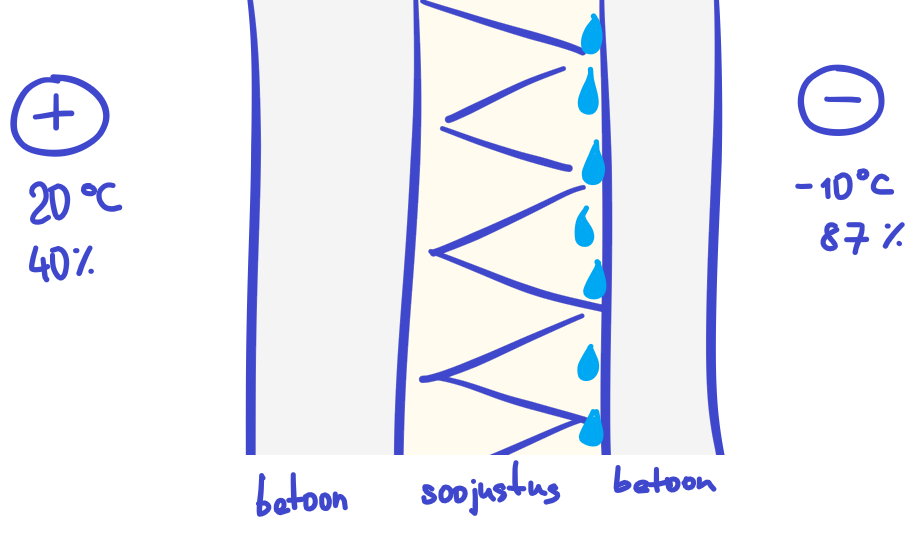
\includegraphics[width=.8\textwidth]{figures/problem_statement/07_layered_structure_sample.png}
    \caption[Mitmest kihist koosneva ehituskonstruktsiooni näide]{\textit{Kihilise konstruktsiooni näide}}
    \label{fig:construction_sample}
\end{figure}

Sellises olukorras kõige olulisemad materjalide omadused on soojuserijuhtivus \begin{math}\lambda\end{math} [W/mK]
ja veeaurutakistus, mis võib olla väljendatud mitmel viisil (viise on palju, aga käesolevas töös keskendutakse 
ainult ühele, kuna see on kõige enam kasutatud nii teadusallikates, kui ka ehitusmaterialide dokumentides):
\begin{math}\mu\end{math} - diffusioonitakistustegur \cite{building_physics_abc}. Infosüsteemi andmemudeli projekteerimisel tuleb kohe arvesse võtma
võimalust lisada tulevikus materjalile ka muud omadused, mis on tarvis teiste tööriistade arendamiseks.

Teatud tingimustel võib tekkida olukord, kui konstruktsiooni ristlõikes on mingis punktis suhteline niiskus
piisavalt kõrge, et soodustada kondensaadi tekkimist \cite{building_physics_abc}. Nimetatud olukord on ohtlik
nii ehituskonstruktsioonile, mis võib pikaajalise niiskuse mõjul laguneda, kui ka inimese tervisele, sest konstruktsioonide
sees tekkiv hallitus on siseruumide õhku sattuvate bakterite allikaks  \cite{building_physics_abc}. 
Seda, kuidas konstruktsioonis toimuvad niiskuse leviku protsessid sõltuvalt materjalide omadustest ja 
paiknemisest ning ümbritsevatest tingimustest, nimetatakse konstruktsiooni niiskustehniliseks toimivuseks. Arvutust,
mille abil võib neid protsesse modelleerida ja kondenseerumise riski hinnata, nimetatakse niiskustehnilise toimivuse
analüüsiks.

Tegemist on klassikalise ehitusfüüsika ülesandega, mille lehandemiseks peab ette võtma järgmiseid samme \cite{iso_13788}:
\begin{itemize}
    \item konstruktsiooni kihtide soojustakistuse ja konstruktsiooni summaarse soojustakistuse arvtus
    \item temperatuuri jaotuse määramine kihtides sõltuvalt sise- ja väliskeskkonna temperatuuridest ning 
    soojustakistuste väärtustest
    \item konstruktsiooni kihtide veeaurutakistuse ja konstruktsiooni summaarse veeaurutakistuse arvutus
    \item veeauru küllastusrõhu jaotuse määramine lähtuvalt temperatuuri jaotusest
    \item veeauru osarõhu jaotuse määramine kihides sõltuvalt sise- ja väliskeskkonna parameetritest ning 
    veeaurutakistuse väärtustest
    \item tulemuste esitamine graafiliselt diagrammil
    \item arvutuste kordamine erinevate sise- ja väliskeskkonna parameetrite kombinatsioonidega
\end{itemize}

Lahendades ülesannet käsitsi, kasutatakse tabeli meetodit: koostatakse tabel, mille ridadesse pannakse 
kirja konstruktsiooni kihid ja veergudesse arvutatakse samm sammult väärtused. 
Kuigi arvutused ei ole keerulised (valemid nimetatud arvutuste teostamiseks on 
leitavad viide-tud allikatest [\colorbox{BurntOrange}{ToDo}]), paraku käsitsi arvutamine 
võtab palju aega, kuna igasugune muudatus (kihi lisamine või järjekorra muutmine) tähendab 
kogu tabeli ümber arvutamist. Pildil \ref{fig:excel_table_sample} on toodud arvutustabel tabeli näide
seitsmest kihist koosneva konstruktsiooni puhul.

\begin{figure}[ht]
    \centering
    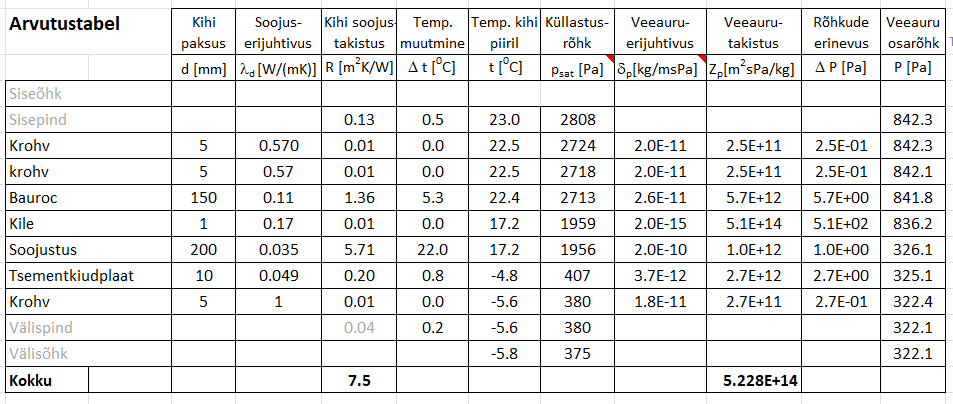
\includegraphics[width=1\textwidth]{figures/problem_statement/04_calc_table.png}
    \caption[Näide niiskustehnilise analüüsi tulemuste esitamisest tabelis]{\textit{Arvutustabeli näide}}
    \label{fig:excel_table_sample}
\end{figure}

Analüüsi tulemused esitatakse graafiliselt diagrammi kujul, mille \begin{math}x\end{math} teljel väärtused on 
punkti asukoht konstruktsiooni ristlõikes ning \begin{math}y\end{math} teljel on temperatuuri, veeauru küllastus- ja
osarõhu väärtused vastavas punktis -- näide diagrammilt on todud pildil  \ref{fig:excel_graph_sample}.

Graafik annab head visuaalset ülevaadet konstruktsiooni kihtides toimuvale. Täpsemalt öeldes, peab vaatama 
veeauru küllastus- ja osarõhkude jaotuse graafikuid. Veeauru osarõhk iseloomustab veeauru tegelikku kontsentratsiooni
teatud punktis, küllastusrõhk iseloomustab veeauru konstentratsiooni, mille ületades hakkab veeaur kondenseeruma.
Veeauru osa- ja küllastusrõhu suhe on suhteline niiskus. Mida lähedam osarõhu graafiku joon küllastusrõhu graafiku 
joonele, seda kõrgem on suhteline niiskus. Punkt, milles need jooned ristuvad on suhteline niiskus 100\%, mis 
tähendab kondensaadi tekkimist -- sellist punkti nimetatakse kastepunktiks konstruktsioonis.
Näide on toodud pildil \ref{fig:excel_graph_sample}: vasakul on niiskustehniline olukord hea, kuna aurutõke asub õiges 
kohas ning seetõttu osarõhk on konstruktsiooni ristlõige kogu ulatuses jääb küllastusrõhult turvaliselt allapoole.
Parempoolsel pildil paikneb konstruktsiooni külmemal pool veeaurutihe kiht, mille tõttu läheb osarõhk kõrgeks ning 
ületab küllastusrõhu väärtust. Tsoonis, kus osarõhk on küllastusrõhust kõrgem, esineb kondensaadi tekkimise oht (pildil
tsoon on viirutatud helesinisega).

\begin{figure}[ht]
    \centering
    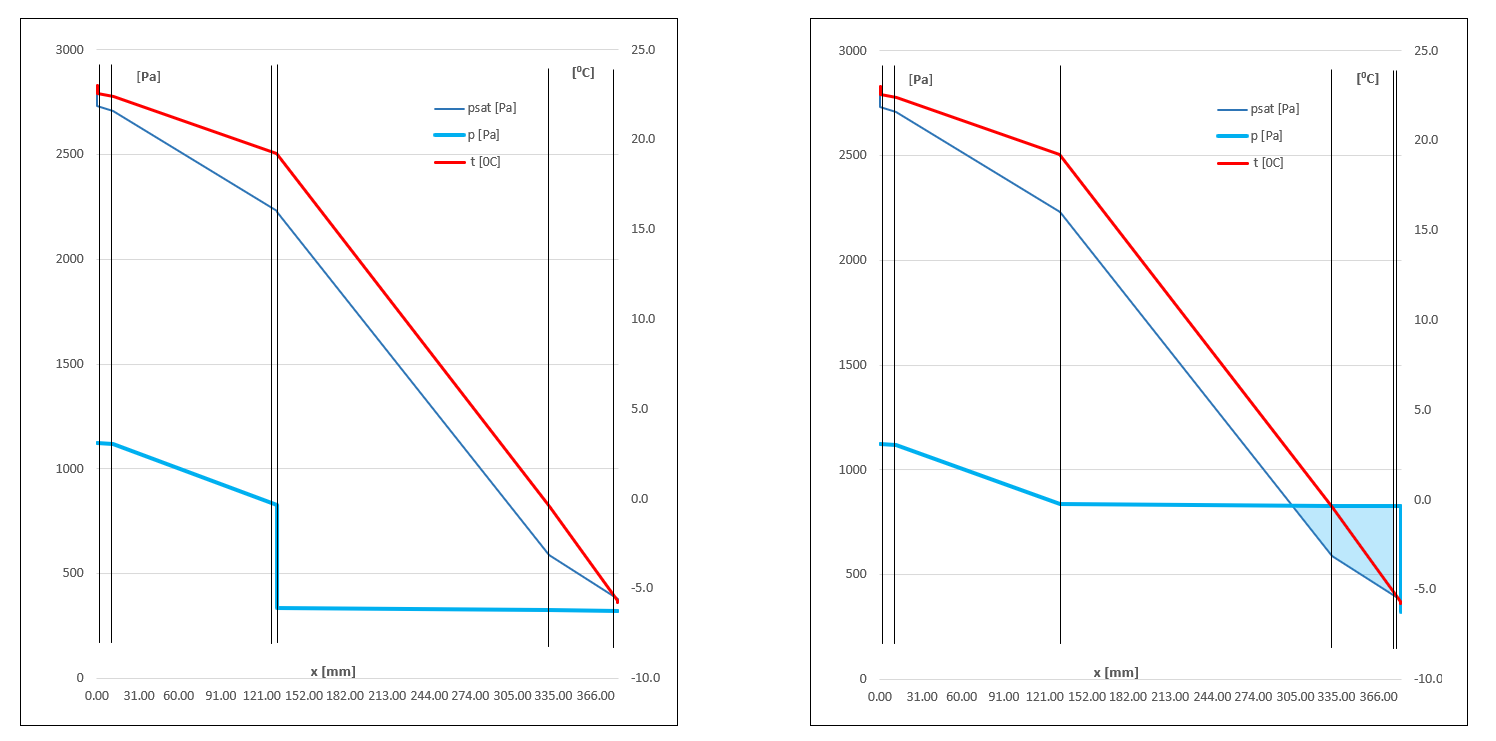
\includegraphics[width=.8\textwidth]{figures/problem_statement/05_excel_grafic_sample.png}
    \caption[Näide niiskustehnilise analüüsi tulemuste esitamisest graafikul]{\textit{Näide tulemuste esitamisest graafikul}}
    \label{fig:excel_graph_sample}
\end{figure}

Kuigi probleem on lahendatav näiteks \textit{Microsoft Excel} vahenditega, paraku pole see kõige mugavam viis
mitmel põhjusel. Selline lähenemine vajab palju käsitööd kihtide lisamiseks või ümber paigutamiseks, mis on analüüsi lahutamata
osa -- proovitakse erinevaid materjale erinevates konstruktsiooni kohtades. Lisaks sellele, näidatud arvutus kehtib vaid ühe 
välisõhu parameetrite kombinatsiooni puhul (temperatuur ja suhteline niiskus), ülevaatliku pildi saamiseks olukorda peab hindama
 aasta lõikes, mis tähendab, et  peab arvutust kordama iga kuu kliimaandmetega.

\section{Olemasolevad lahendused}
\label{chapters:problem_statement_existing_solutions}
Üks populaarsematest analoogsetest lahendustest, mis on inseneridel kasutusel Euroopas, sealhulgas ka Eestis, on Saksa päritoluga tarkvara \textbf{Ubakus}. 
Tegemist on kommertstarkvaraga, mis töötab veebirkenduse kujul. Tarvara \textit{demo}-versioon on saadaval tasuta.
\begin{figure}[ht]
    \centering
    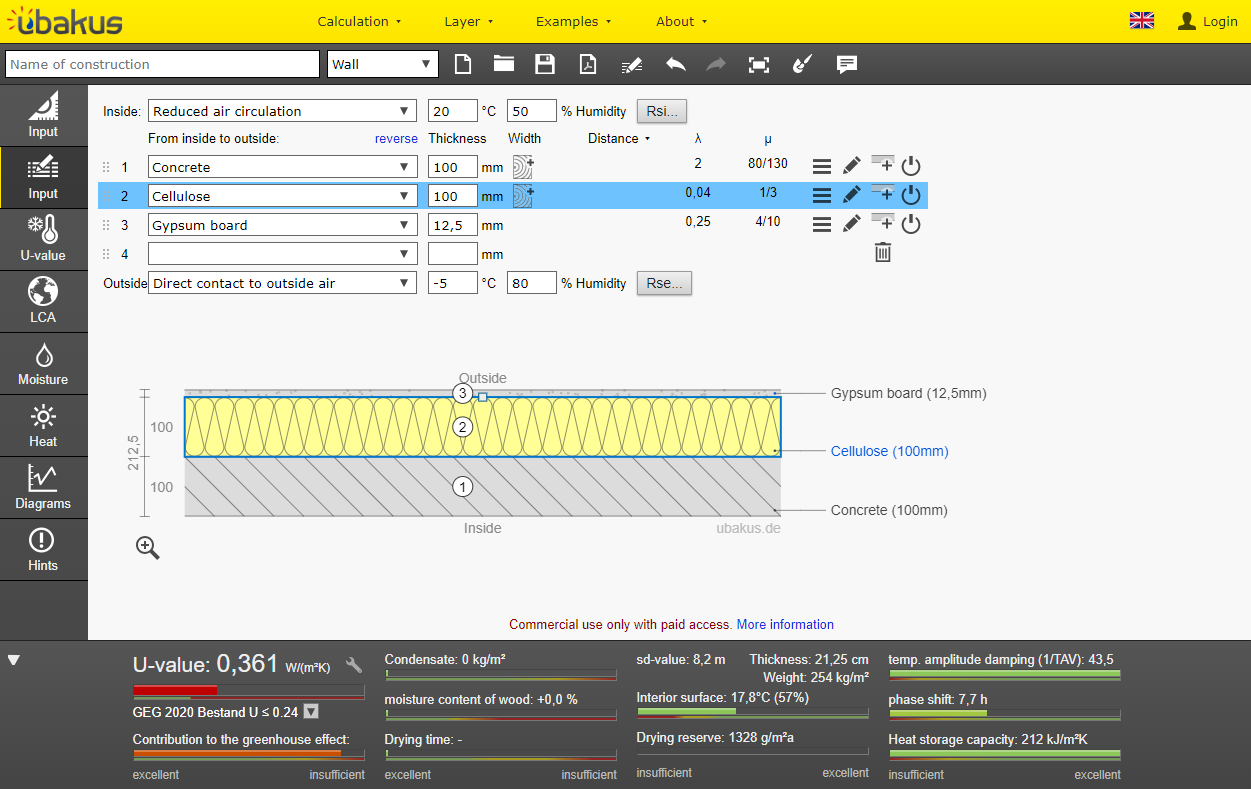
\includegraphics[width=1\textwidth]{figures/problem_statement/01_ubakus.png}
    \caption[Ubakus tarkvara katutajaliides, ekraanitõmmis]{\textit{Ubakus: kasutajaliides, ekraanitõmmis.}}
    \label{fig:ubakus_sample}
\end{figure}

\textbf{Ubakus} võimaldab teostada konstruktsiooni niiskustehnilist analüüsi. Kasutajaliides võidaldab 
mudeldada mitmest kihist koosneva konstruktsiooni, valides igale kihile paksust ja materjali, millest 
kiht koosneb. Tugev eelis on see, et tarkvaraga saab analüüsida ka mittehomogeensete (mitemest erinevast 
materjalist, nt puitsõrestiksein) kihtidega konstruktsioone -- pilt \ref{fig:ubakus_sample} \cite{ubakus}.

Ehitusmaterjalide valik, mida on võimalik konstruktsiooni mudeldamisel kasutada, on piisavalt lai 
(aga tasuta versioonis piiratud). Tasulises versioonis on samuti võimalik ka oma materjalide 
lisamine ja kasutamine. Osa materjalidest on abstraktsed (näiteks: betoon, puit, mineraalvill), osa
on reaalsed turustatavad tooted (näiteks: Isover soojusisolatsioonide valik) -- pilt \ref{fig:ubakus_materials}. Võib puuduseks pidada
seda, et osa materjale (konkreetsed toted) on Saksamaal ja Kesk-Euroopas turustatavad materjalid, mistõttu selle 
tarkvara kasutades Eestis peab kas sisestama vajalikud kohalikud materjalid käsitsi, või arvestada Saksa analoogide
kasutusest tuleneva arvutuste ebatäpsusega.
\begin{figure}[ht]
    \centering
    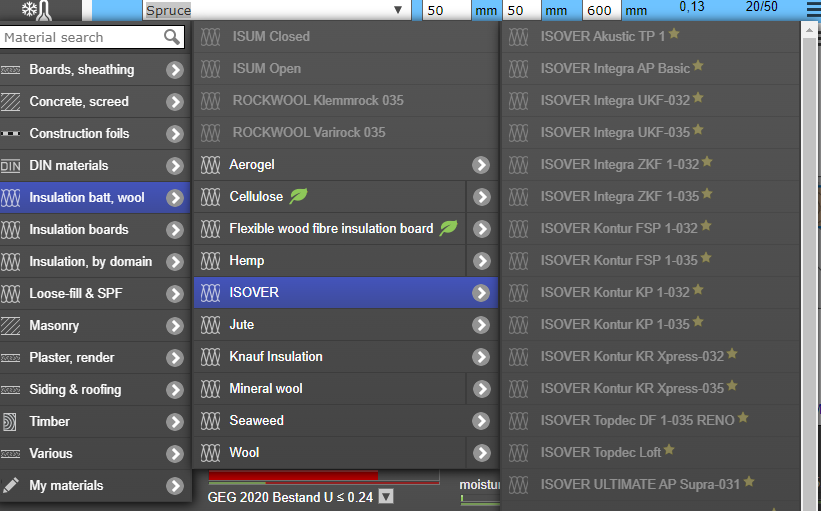
\includegraphics[width=1\textwidth]{figures/problem_statement/03_ubakus_materials.png}
    \caption[Ubakus tarkvara materjalide valik, ekraanitõmmis]{\textit{Ubakus: ehitusmaterjalide valik baasis, ekraanitõmmis.}}
    \label{fig:ubakus_materials}
\end{figure}

Keskkonnatingimused valitakse manuaalselt sisestades õhutemperatuuri ja -niiskuse väärtused. Rakendus võimaldab arvutuste tulemust
vaadata erineval viisil, alates lihtsamast 3D visualiseeringust kuni värvilise temperatuurikaardini. Tarkavara saab osa aastase 
tellimusega, mille maksumus on alates 50 kuni 120 eurot sõltuvalt valitud paketist. Objektiivselt vaadates on tarkvara hea nii
funktsionaalsuse kui ka hinna seisukohalt. Lisaks sellele on ka kasutajaliides piisavalt mugav ja intuitiivselt arusaadav,
et seda saaks kasutada ka inimene, kellel puuduvad sügavad teadmised valdkonnast. Nagu varem oli mainitud, 
takvara on suunatud eelkõige Kesk-Euroopa ja Canada turgudele, Balti ja Skandinaavia riigidele lokaliseerimine puudub. Kokkuvõttes
antud lahendust võib kindlasti võtta arvesse toote funktsionaalsuse kavandamisel.

\textbf{Physibel Glasta} on üks analoogne lahendus veel, mis on samuti kommertstarkvara. Tegemist on samuti arvutile paigaldatava tarkvaraga, mille
kasutajaliides on veidi keerulisem ja ka disain on oluliselt konservatiivsem (pilt \ref{fig:glasta_sample}) \cite{glasta}. 
\begin{figure}[ht]
    \centering
    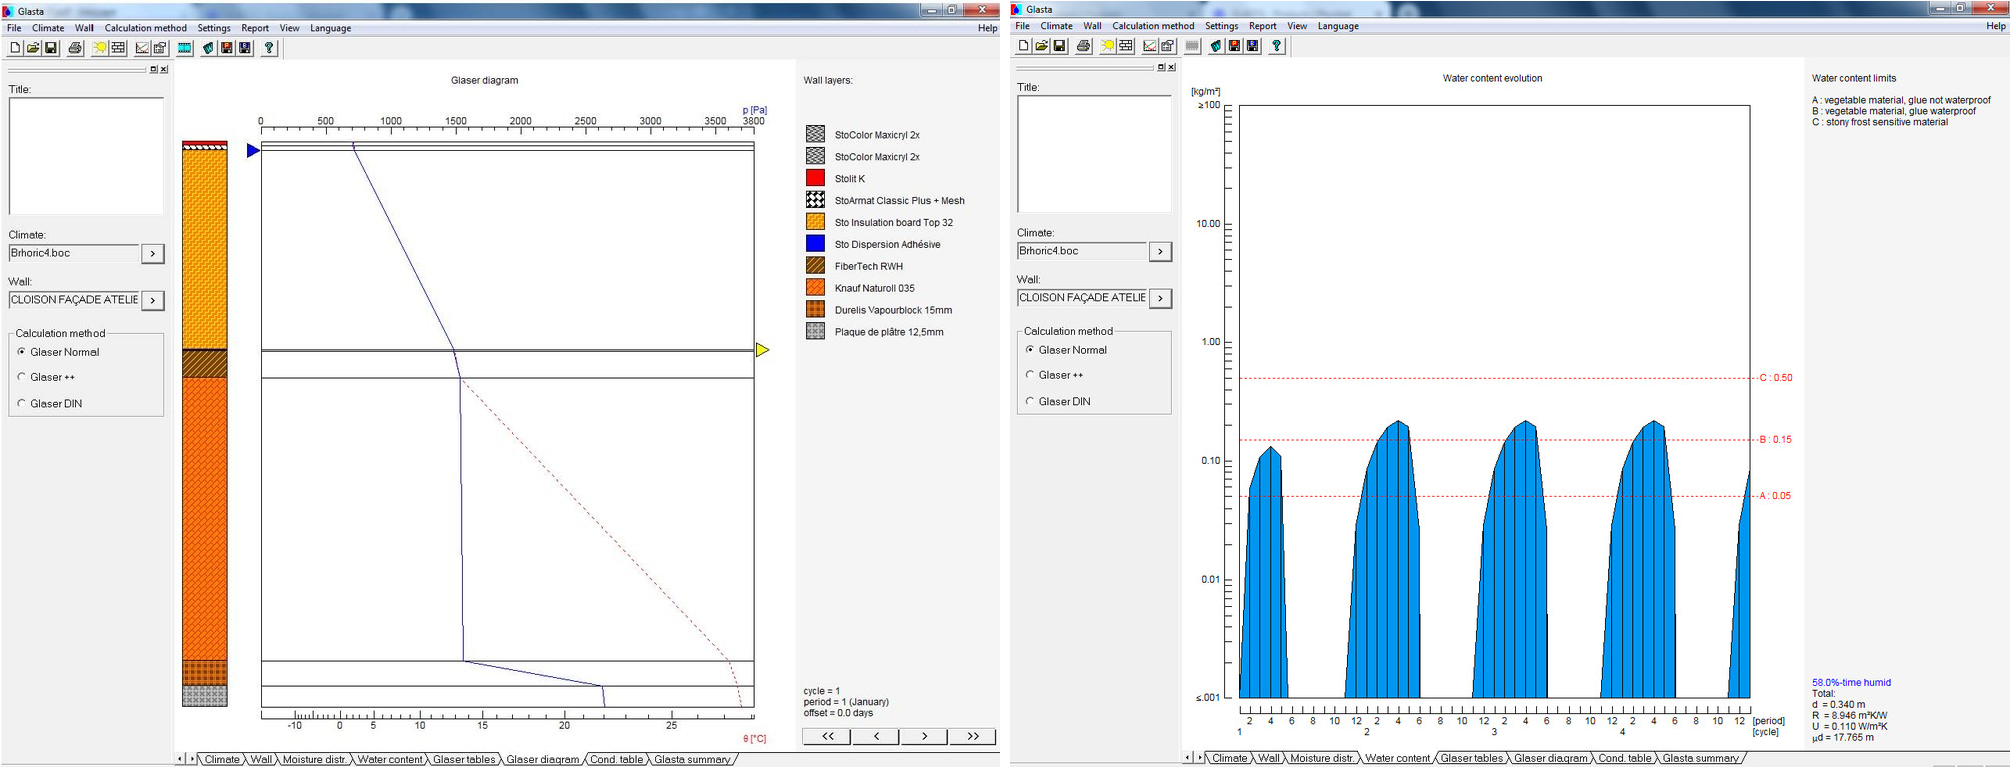
\includegraphics[width=1\textwidth]{figures/problem_statement/09_glasta_sample.png}
    \caption[Physibel Glasta tarkvara kasutajaliides, ekraanitõmmis]{\textit{Glasta: kasutajaliides, ekraanitõmmis.}}
    \label{fig:glasta_sample}
\end{figure}

Selle tarkvara funktsionaalsuse tugev eelis on võimalus teostada analüüsi aasta lõikes - väga tihti 
kondenseerumise probleem esineb vaid teatud perioodil (tavaliselt külmal hooajal),
ülejäänud ajal toimub kuivamine. See, et ühel või kahel talvisel kuul esineb konstruktsioonis kondenseerumise oht ei pruugi
olla probleemiks, kui ülejäänud ajal jõuab konstruktsioon täielikult kuivada. Antud asjaolu Glasta tarkvara analüüsib ning 
tulemust esitatakse ka graafikul (pilt \ref{fig:glasta_sample}). Antud funktsionaalsus on äärmiselt oluline ja selle vajadusega peab toote 
planeerimisel arvestama. Tarkvara hind on suurusjärgus 500 eurot aastas, mis on päris kõrge, ning lisaks ka alla laadimise ja 
paigaldamise vajadus teeb antud lahendust ebamugavaks ja paljudel juhtudel ebaotstarbekaks.

Valdkonnas on olemas ka oma lipulaev -- \textbf{Delphin} on professionaalne tarkvara, mille hind on suurusjärgus 1000-1500 eurot aastas \cite{delphin}.
Eelisteks on väga lai funktsionaalsus ning ka täielik vabadus konstruktsiooni mudeldamisel. Erineval eeltoodu analoogidest,
tarkvara võimaldab koostada ja analüüsida konstruktsiooni sõlme. Samuti on tarkvaras võimalik mudeldada analüüsi lähteandmeteks olevad
ilmaandmed. Tavakasutaja jaoks viimane on ühtlasi ka puuduseks, sest kliimatingimuste mudeldamine eeldab ilmatingimuste 
(sealhulgas ka andmed päikesekiirgusest, sademetest) andmebaasi olemasolu. Samuti vajab tarkvara ka kasutaja koolitust, 
mida tootja pakub ka pakub hinnaga 800 eurot. Eeltoodud asjaolud teevad antud tarkvara sobilikuks ja otstarbekaks
nendele, kellel ehitusfüüsika arvutused on põhitegevuseks (nt tarkvara on laialt kasutusel teadusvaldkonnas). 

\begin{figure}[ht]
    \centering
    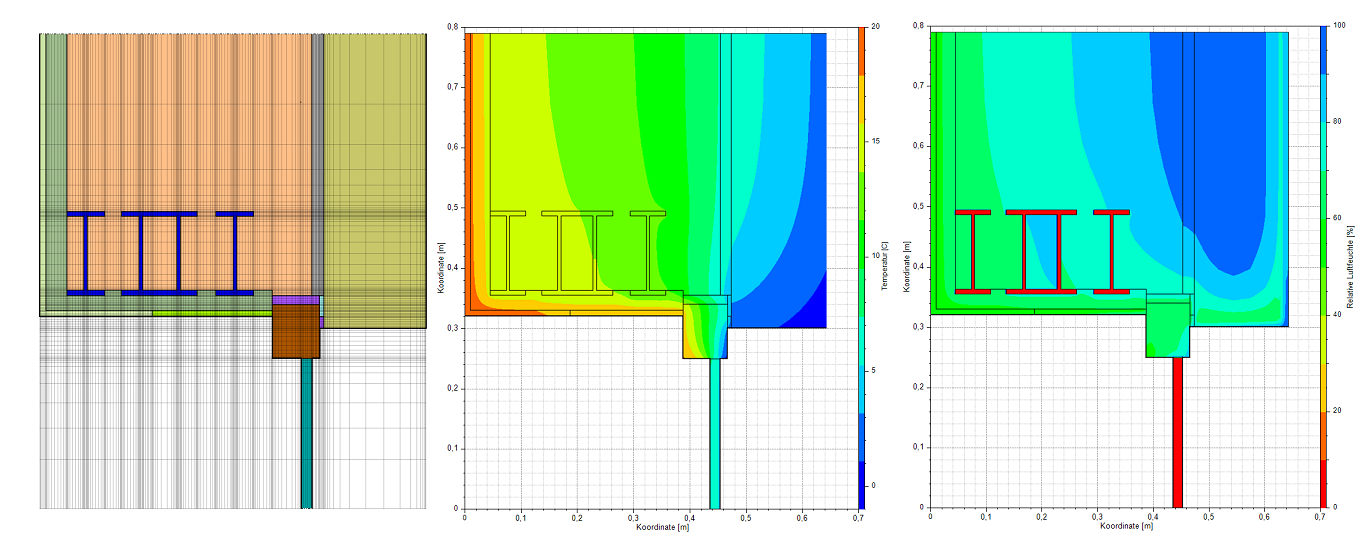
\includegraphics[width=1\textwidth]{figures/problem_statement/08_delphin_sample.png}
    \caption[Delphin tarkvara kasutajaliides, ekraanitõmmis]{\textit{Delphin: kasutajaliides, ekraanitõmmis.}}
    \label{fig:delfin_sample}
\end{figure}

